\section{Introduction}
\subsection{Project background and scope}
In many applications, primarily in agriculture, an autonomous UAV which can follow a pre programmed route and return to a base to recharge like an autonomous lawn mower, is sought after. One case could be a farmer. As the legislation is now the farmer must daily inspect his animals. This prevents the use of some remote areas which is otherwise perfect for the farmer’s use; as small islands or remote field with good grass. Areas that take time, money or effort to get to in order to inspect the animals.
Our vision is to develop a system which allows a UAV to take off, fly a pre programmed route if conditions allow flying, return to the base by GPS and the guided via GNSS/computer vision land to recharge on a ground base. Then the UAV will be ready for next flight the next day.
\subsection{Problem formulation}
The problems in this project will be to:

\begin{itemize}
	\item Modify Pixhawk firmware to be controlled automatically from an external computer;
	\item Build/design/construct a landing-platform with mechanical autofit;
	\item Design a tracking-system that outputs 3D-positions; and,
	\item Design a program that analyze 3D-positions and outputs control-signals.
\end{itemize}

\subsection{Related work}
We found a project done by Weiwei Kong, Daibing Zhang, Xun Wang, Zhiwen Xian and Jianwei Zhang, researchers at National University of Defence Technology in Changsha, China and University of Hamburg. This study used a stereo infrared setup placed on the ground which is then used to guide a UAV (multirotor or fixed wing) to land in a designated area. The idea of this is the same as ours, though for our use it does not need to be equipment this expensive. Also we do not need the flexibility they get by having a remote camera. What we need is precision and we also always have the same aircraft to guide. But in general the idea is the same, a ground based guidance system for landing. The article can be found at \url{http://ieeexplore.ieee.org/xpls/abs_all.jsp?arnumber=6696776&tag=1}

\subsection{Aim}
The group will focus on the ground base, landing system and guidance of the drone. We decided to use a IRIS-UAV which is controlled by a pixhawk and then modify the landing gear to fit our concept. We will not develop a charging system as there are already plenty of these, but we will show connectivity and thereby simulate charging.
 
The GNSS is not expected to be precise enough for landing on the platform. It will mainly be used to guide the UAV back in the region of the landing platform. In this region a camera in the landing platform will start tracking the position of the UAV. The landing platform will then take control of the UAV (by telemetry), and start landing the drone based on the vision tracking.
\begin{figure}
	\centering
	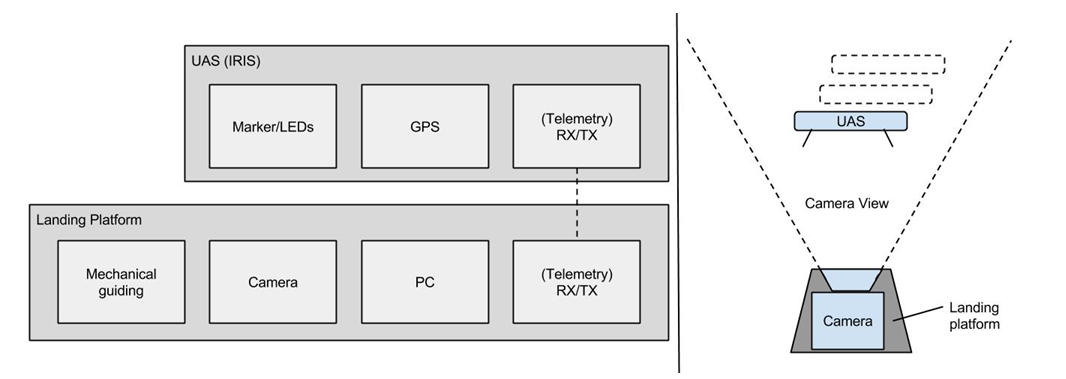
\includegraphics[width=0.8\textwidth]{imgs/introduction}
	\caption{Basic idea of how the system could be build}
\end{figure}